\documentclass[11pt]{article}

% ---------------------------------------------------------------- packages
\usepackage[utf8]{inputenc}
\usepackage[T1]{fontenc}
\usepackage{amsmath,amssymb,amsthm}
\usepackage{graphicx}
\usepackage{booktabs}
\usepackage{geometry}
\usepackage{caption}
\usepackage{subcaption}
\usepackage{xcolor}
\usepackage[hidelinks]{hyperref}
\usepackage{natbib}
\usepackage{authblk}

\geometry{margin=1in}
\graphicspath{{../results/figures/}{./figures/}}

% Long unbreakable runs (inline math, \texttt paths) otherwise push a few lines
% past the right margin.  emergencystretch lets TeX relax interword spacing on a
% final pass instead of overflowing; it changes nothing where lines already fit.
\emergencystretch=3em

% ---------------------------------------------------------------- submission
% FILL IN BEFORE SUBMISSION.  While these still read "TO BE INSERTED",
% `python scripts/build_paper.py --check` reports the paper as not
% submission-ready, because the Code-availability statement below promises a
% location a referee cannot reach.
% These five fields are managed from paper/metadata.json by
% `python scripts/set_metadata.py`; edit that file, not these lines, then
% rerun the script to inject the values and rebuild the PDF.
\newcommand{\coderepo}{\url{https://github.com/Raahul-Thakur/optimal-portfolio-rebalancing}}
\newcommand{\codedoi}{[ARCHIVED DOI TO BE INSERTED]}
\newcommand{\authororcid}{\url{https://orcid.org/0009-0000-9506-0628}}
\newcommand{\affiliation}{Birla Institute of Technology and Science, Pilani, India}

\newtheorem{proposition}{Proposition}
\newtheorem{remark}{Remark}
\newcommand{\E}{\mathbb{E}}
\newcommand{\R}{\mathbb{R}}
\newcommand{\half}{\tfrac{1}{2}}

% ---------------------------------------------------------------- title
\title{\bfseries A Variational Control Framework for Optimal Portfolio
Rebalancing Under Transaction Costs}
\author[1]{Rahul Thakur}
\affil[1]{\normalsize \affiliation}
\affil[ ]{\normalsize\texttt{raahul.thakurr01@gmail.com}}
\date{November 2026}

\begin{document}
\maketitle

% ================================================================ Abstract
\begin{abstract}
\noindent
We study portfolio rebalancing between one risky and one risk-free asset as a
finite-horizon stochastic control problem with proportional transaction costs
and constant-relative-risk-aversion (CRRA) preferences. Exploiting the
homogeneity of CRRA utility we reduce the value function to a one-dimensional
object in the risky-allocation fraction and solve the Bellman recursion exactly
(to quadrature and grid resolution) by backward induction. The solution
reproduces the classical \emph{no-trade region}: a band of allocations around
the frictionless Merton target inside which it is optimal not to trade, and
toward whose boundary the investor trades when outside. We confirm the textbook
comparative statics --- the band widens with the transaction-cost rate
(consistent with the small-cost $tc^{1/3}$ scaling) and narrows with risk
aversion --- and the horizon effect by which the band flares open near the
terminal date.

We then ask a computational question: can a lightweight neural network imitate
this optimal control? Training a $4{,}417$-parameter multilayer perceptron by
supervised regression on the dynamic-programming policy attains a validation
mean-squared error of $2.1\times10^{-4}$, yet a paired Monte-Carlo evaluation
(common random numbers, $20{,}000$ paths) shows the learned policy is the
\emph{worst} performer by certainty equivalent. The mechanism is structural: a
smooth regressor cannot represent the exact ``do nothing'' identity on a
positive-measure set, so its tiny action-space errors inside the no-trade region
are amplified into continuous spurious turnover (mean turnover $0.21$ versus
$3\times10^{-5}$ for the optimal policy). We then show the diagnosis is
actionable: restoring the inaction region --- by a dead-zone wrapper at
inference, or by penalizing excess turnover during training --- closes the
entire certainty-equivalent gap, leaving the repaired network statistically
indistinguishable from the optimal control ($t=-0.4$, against $t=20.1$ before
the repair). Recovery sets in precisely as the dead-zone width crosses the
network's in-band residual, confirming the mechanism. Both the failure and its
repair are robust: across $10$ seeds and $7$ architectures spanning a factor of
$198$ in capacity, every student over-trades and under-performs, the largest
network has the \emph{worst} in-band residual, and the dead-zone recovers the
optimum in all $17$ cases. We conclude that imitating optimal \emph{control}
requires encoding the inaction region rather than minimizing action-space error.
All results are reproducible from the accompanying code.
\vspace{0.6em}
\noindent\textbf{Keywords:} portfolio rebalancing; transaction costs; no-trade
region; stochastic control; dynamic programming; imitation learning;
reproducible research.

\vspace{0.3em}
\noindent\textbf{JEL classification:} G11; C61; C63; C45.
\end{abstract}

% ================================================================ Intro
\section{Introduction}

\subsection{Motivation}
A long-only investor who wants to hold a fixed fraction of wealth in a risky
asset faces a basic tension. Random returns continuously perturb the realized
allocation away from the target, but every corrective trade costs money. In a
frictionless world the resolution is trivial: rebalance continuously to the
\citet{merton1969} target. With transaction costs, continuous rebalancing is
infinitely expensive, and the optimal policy instead tolerates deviations,
trading only when the allocation drifts too far. Characterizing ``too far'' is
the heart of the problem.

\subsection{Transaction costs and rebalancing}
Proportional transaction costs transform the single optimal allocation point
into an interval of inaction --- the \emph{no-trade region}. This qualitative
feature, first identified by \citet{magillconstantinides1976} and rigorously
established by \citet{constantinides1986}, \citet{davisnorman1990} and
\citet{shrevesoner1994}, is robust across model specifications and is the single
most important practical consequence of trading frictions. Its width encodes the
cost--benefit trade-off of rebalancing and directly governs realized turnover.

\subsection{Research questions}
This paper is deliberately \emph{reproductive and computational} rather than
model-innovative. We pursue three questions.
\begin{enumerate}
  \item[\textbf{Q1.}] Does a transparent, discrete-time dynamic program recover
  the classical no-trade region and its comparative statics?
  \item[\textbf{Q2.}] Can a small neural network, trained by supervised
  imitation of the optimal policy, serve as a fast approximate controller?
  \item[\textbf{Q3.}] How do the optimal policy, its learned approximation, and
  simple heuristics (periodic rebalancing, buy-and-hold) compare on economic
  performance, turnover, and cost?
\end{enumerate}
Our contributions are (i) a clean, fully reproducible discrete-time solver that
exploits CRRA homogeneity for a one-dimensional state; (ii) a closed-form
proportional-cost wealth-update identity that makes the recursion exact and
vectorizable; and (iii) the finding that naive action-space imitation
\emph{systematically fails} by violating the no-trade region, with a clear
mechanistic explanation and statistically rigorous paired evidence.

% ================================================================ Lit
\section{Literature Review}

\paragraph{Portfolio optimization.}
\citet{merton1969,merton1971} solved the frictionless dynamic
consumption--investment problem, giving the constant optimal risky weight
$w^{*}=(\mu-r)/(\gamma\sigma^2)$ that anchors our no-trade region.

\paragraph{Transaction-cost models.}
\citet{magillconstantinides1976} introduced proportional costs and the no-trade
region concept; \citet{constantinides1986} quantified its asset-pricing
implications; \citet{davisnorman1990} and \citet{shrevesoner1994} provided the
singular-control and viscosity-solution foundations, including the small-cost
asymptotics in which the half-width of the band scales like $tc^{1/3}$.
\citet{dumasluciano1991} obtained an exact infinite-horizon solution, and
\citet{kallsenmuhlekarbe2010} developed the shadow-price approach.
\citet{liu2004} extended the analysis to multiple risky assets and
\citet{garleanupedersen2013} to predictable returns under quadratic costs.

\paragraph{Dynamic programming.}
The backward-induction machinery we use is standard \citep{bertsekas2017}; our
only specialization is the homogeneity reduction that collapses the state to the
allocation fraction.

\paragraph{Learning-based portfolio control.}
Machine learning has been applied to high-dimensional control via deep
BSDE/PDE solvers \citep{hanjentzene2018} and to hedging under frictions via deep
hedging \citep{buehler2019deephedging}. We instead study the simplest learning
paradigm --- supervised \emph{imitation} of a known optimal controller
\citep{rossbagnell2011,suttonbarto2018} --- precisely to isolate when and why it
fails. Our negative result complements the deep-hedging literature by showing
that the inaction structure induced by transaction costs is exactly what naive
imitation cannot represent.

% ================================================================ Framework
\section{Mathematical Framework}
\label{sec:framework}

\subsection{Market model}
Time is discrete, $t=0,1,\dots,N$, with step length $dt=T/N$. The risky asset
price $S_t$ follows a discrete-time geometric Brownian motion, so its one-step
gross return is
\begin{equation}
R_{t+1}=\frac{S_{t+1}}{S_t}
=\exp\!\Big((\mu-\half\sigma^2)\,dt+\sigma\sqrt{dt}\,Z_{t+1}\Big),
\qquad Z_{t+1}\stackrel{\text{iid}}{\sim}N(0,1),
\label{eq:gbm}
\end{equation}
with drift $\mu$ and volatility $\sigma$. The risk-free asset grows
deterministically by $R_f=e^{r\,dt}$. Equation~\eqref{eq:gbm} implies the
lognormal moments $\E[R]=e^{\mu\,dt}$ and $\E[R^2]=e^{2\mu\,dt+\sigma^2 dt}$,
which we use to validate the quadrature in Section~\ref{sec:numerics}.

\subsection{Wealth, state, and control}
At date $t$, before trading, the investor holds $A_t$ dollars in the risky asset
and $C_t$ in cash, with total wealth $W_t=A_t+C_t$ and risky fraction
$x_t=A_t/W_t$. The control is the \emph{post-trade} risky fraction
$y_t\in[0,1]$ (no shorting, no leverage). The pair $(W_t,x_t)$ is the state and
$y_t$ the action.

\subsection{Transaction costs and the wealth-update identity}
\label{sec:tc}
Normalize $W_t=1$ (justified below). Pre-trade holdings are $A=x$ in risky and
$1-x$ in cash. Choosing post-trade fraction $y$ requires trading
$\delta$ dollars into the risky asset; the proportional cost $tc\,|\delta|$ is
paid from cash, so post-trade wealth is $m=1-tc\,|\delta|$ and the post-trade
risky holding is $y\,m=A+\delta$, i.e. $\delta=ym-x$. Substituting
$m=1-tc|\delta|$ and solving the resulting fixed point yields a closed form.

\begin{proposition}[Proportional-cost wealth multiplier]
\label{prop:m}
For $tc\in[0,1)$ and $x,y\in[0,1]$, the post-trade wealth multiplier is
\begin{equation}
m(x,y)=
\begin{cases}
\dfrac{1+tc\,x}{1+tc\,y}, & y\ge x \quad(\text{buying}),\\[2.2ex]
\dfrac{1-tc\,x}{1-tc\,y}, & y< x \quad(\text{selling}),
\end{cases}
\label{eq:m}
\end{equation}
and the traded amount satisfies $\delta=(y-x)/(1\pm tc\,y)$, so
$\operatorname{sign}(\delta)=\operatorname{sign}(y-x)$ and $m(x,x)=1$.
\end{proposition}

\begin{proof}
If $\delta>0$ (buying), $m=1-tc\,\delta$ and $\delta=ym-x$. Then
$m=1-tc(ym-x)\Rightarrow m(1+tc\,y)=1+tc\,x$, giving the first branch.
Substituting back, $\delta=ym-x=(y-x)/(1+tc\,y)>0$ iff $y>x$, confirming the
case split. The selling branch ($\delta<0$) is symmetric with $m=1+tc\,\delta$,
yielding $m(1-tc\,y)=1-tc\,x$ and $\delta=(y-x)/(1-tc\,y)$. At $y=x$ both
branches give $m=1$ and $\delta=0$.
\end{proof}

Equation~\eqref{eq:m} is exact (no linearization) and renders the entire
recursion a handful of vectorized array operations.

\subsection{Preferences and the Bellman recursion}
The investor maximizes expected terminal CRRA utility
\begin{equation}
U(W)=\frac{W^{1-\gamma}}{1-\gamma},\qquad \gamma>0,\ \gamma\ne 1,
\end{equation}
with relative risk aversion $\gamma$. After trading to fraction $y$ at
normalized wealth $m$, one market step \eqref{eq:gbm} sends wealth to
$W'=m\,\phi(y,R)$ and the fraction to $x'(y,R)$, where
\begin{equation}
\phi(y,R)=yR+(1-y)R_f,\qquad x'(y,R)=\frac{yR}{\phi(y,R)} .
\label{eq:transition}
\end{equation}
The value function $V_t(W,x)=\sup\E[U(W_N)\mid W_t=W,x_t=x]$ obeys
$V_N(W,x)=U(W)$ and
\begin{equation}
V_t(W,x)=\max_{y\in[0,1]}\ \E_R\!\big[V_{t+1}(W',x')\big].
\label{eq:bellman-full}
\end{equation}

\subsection{Dimensionality reduction by homogeneity}
\begin{proposition}[Homogeneity reduction]
\label{prop:homog}
There exist functions $g_t:[0,1]\to\R$ with
$V_t(W,x)=W^{1-\gamma}\,g_t(x)$ for all $t$. They satisfy the one-dimensional
recursion
\begin{equation}
\boxed{\;
g_t(x)=\max_{y\in[0,1]}\ m(x,y)^{1-\gamma}\,
\E_R\!\big[\phi(y,R)^{1-\gamma}\,g_{t+1}\!\big(x'(y,R)\big)\big],
\qquad g_N(x)\equiv\frac{1}{1-\gamma}. \;}
\label{eq:bellman-reduced}
\end{equation}
\end{proposition}

\begin{proof}
By backward induction. At $t=N$, $V_N(W,x)=W^{1-\gamma}/(1-\gamma)$, so
$g_N\equiv 1/(1-\gamma)$. Assume $V_{t+1}(W,x)=W^{1-\gamma}g_{t+1}(x)$. From
Section~\ref{sec:tc}, trading from $(W,x)$ to fraction $y$ gives post-trade
wealth $W\,m(x,y)$, and the market step \eqref{eq:transition} sends wealth to
$W'=W\,m(x,y)\,\phi(y,R)$ with next fraction $x'(y,R)$ independent of $W$.
Then
\[
V_t(W,x)=\max_y\E_R\!\big[(W')^{1-\gamma}g_{t+1}(x')\big]
=W^{1-\gamma}\max_y m(x,y)^{1-\gamma}
\E_R\!\big[\phi(y,R)^{1-\gamma}g_{t+1}(x')\big],
\]
which is $W^{1-\gamma}g_t(x)$ with $g_t$ as in
\eqref{eq:bellman-reduced}. Both $m$ and $x'$ are wealth-independent, so the
maximizer $y^{*}(t,x)$ depends only on $(t,x)$.
\end{proof}

Proposition~\ref{prop:homog} is the workhorse: it removes wealth from the state
space, leaving the scalar allocation fraction $x$ as the only continuous state.

\subsection{The no-trade region}
The optimal policy is $y^{*}(t,x)=\arg\max_y(\cdot)$ in
\eqref{eq:bellman-reduced}. Define the date-$t$ \emph{no-trade region}
\begin{equation}
\mathrm{NT}_t=\{x:\ y^{*}(t,x)=x\}.
\end{equation}
The classical structural result --- which our numerics confirm --- is that
$\mathrm{NT}_t=[\,\underline{x}_t,\ \overline{x}_t\,]$ is an interval around the
Merton target $w^{*}$, with
\begin{equation}
y^{*}(t,x)=
\begin{cases}
\underline{x}_t, & x<\underline{x}_t \quad(\text{buy to lower edge}),\\
x, & x\in[\underline{x}_t,\overline{x}_t] \quad(\text{hold}),\\
\overline{x}_t, & x>\overline{x}_t \quad(\text{sell to upper edge}).
\end{cases}
\label{eq:bangbang}
\end{equation}
Trading is ``bang-bang to the boundary'': when action is warranted, the investor
moves exactly to the nearest edge of the inaction band, never overshooting into
its interior.

% ================================================================ Numerics
\section{Numerical Solution}
\label{sec:numerics}

\subsection{State and action discretization}
We discretize the fraction $x$ on a uniform grid of $n_x=201$ points in
$[0,1]$; the action $y$ shares this grid. The risky-return expectation in
\eqref{eq:bellman-reduced} is evaluated by $n_q=21$-node Gauss--Hermite
quadrature: for $Z\sim N(0,1)$,
$\E[f(R)]\approx\pi^{-1/2}\sum_i w_i\,f\!\big(R(\sqrt2\,z_i)\big)$ with
physicists' nodes $(z_i,w_i)$. This reproduces the lognormal moments of
Section~\ref{sec:framework} to machine precision (relative error
$<10^{-8}$ for $\E[R]$ and $\E[R^2]$).

\subsection{Backward induction and policy extraction}
Starting from $g_N\equiv 1/(1-\gamma)$ we iterate \eqref{eq:bellman-reduced}
backward. For each action $y$ on the grid we precompute the next fractions
$x'(y,R)$ and gross returns $\phi(y,R)$ over the quadrature nodes; the
continuation value $g_{t+1}$ is evaluated at $x'(y,R)$ by linear interpolation.
The cost multiplier $m(x,y)$ from \eqref{eq:m} is a full $(n_x\times n_y)$
matrix, and the objective $J_t(x,y)=m(x,y)^{1-\gamma}\E_R[\cdots]$ is maximized
over $y$ by a vectorized $\arg\max$. The per-step cost is
$O(n_x\,n_y\,n_q)$ and the full $N=52$-step solve completes in $\approx 0.02$\,s.
The no-trade boundaries $\underline{x}_t,\overline{x}_t$ are read off as the
range of $x$ for which $|y^{*}(t,x)-x|$ is within one grid spacing.

\paragraph{The reduced value function.}
Figure~\ref{fig:value} plots the solved $g_t(x)$ at three dates and makes the
geometry of the problem visible. At every date $g_t$ is concave and peaks at
the Merton fraction $w^{*}=0.300$, confirming that the frictionless target
remains the centre of gravity once costs are added. Two features matter for
what follows. First, the level of $g_t$ rises with time-to-go (from
$g_{51}(w^{*})=-0.2494$ to $g_0(w^{*})=-0.2227$, against the terminal value
$g_N\equiv1/(1-\gamma)=-0.25$): a longer horizon is worth more because the
risky premium has longer to compound. Second, and more importantly, the
\emph{curvature} collapses near the horizon --- the spread of $g_t$ across the
whole allocation interval falls from $6.1\times10^{-3}$ at $t=0$ to
$9.4\times10^{-4}$ at $t=51$. A nearly flat value function means the
allocation barely matters, so almost no deviation is worth a trade. This is
the mechanism behind the horizon effect reported in
Section~\ref{sec:results}: the band flares open precisely where $g_t$ goes
flat.

\begin{figure}[t]
\centering
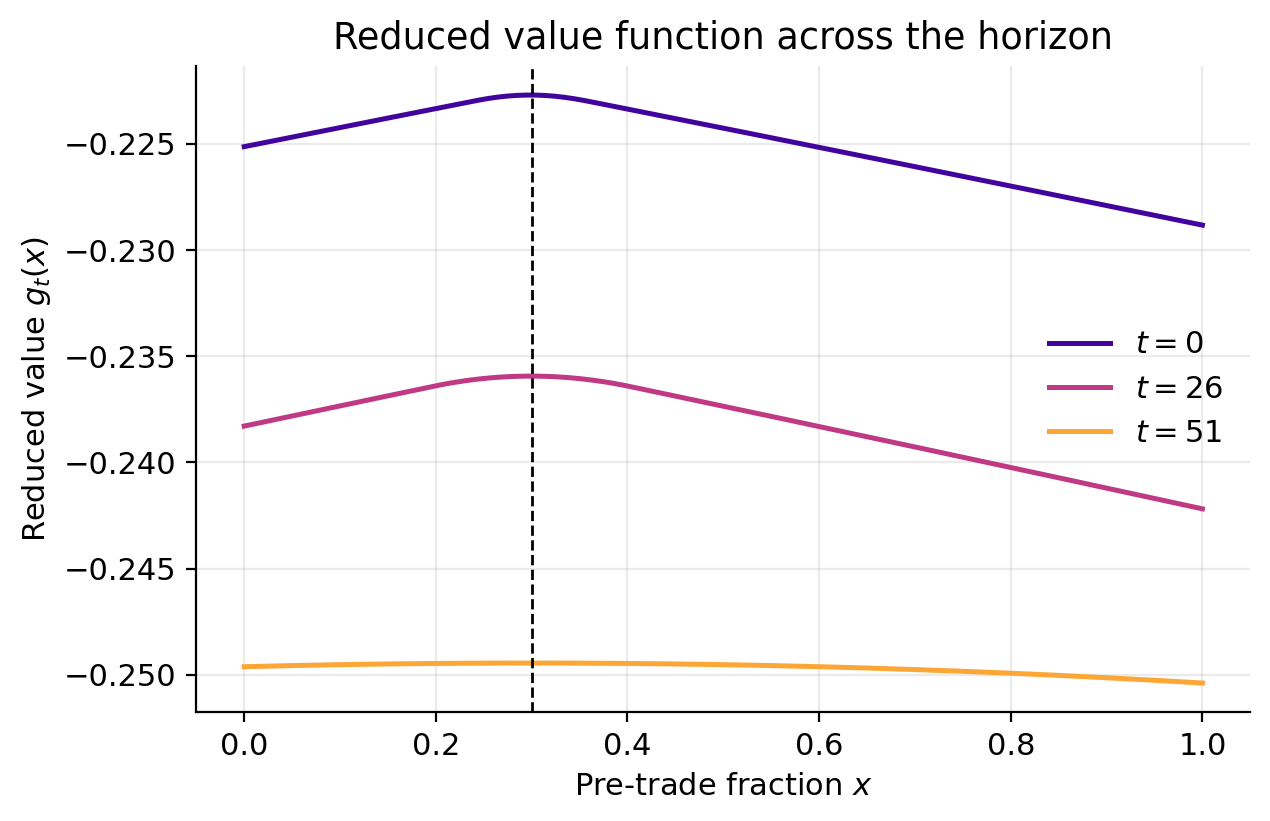
\includegraphics[width=0.72\textwidth]{fig3_value_function.png}
\caption{The reduced value function $g_t(x)$ at $t=0$, $t=26$ and $t=51$
(dashed line: the Merton fraction $w^{*}=0.30$). Each slice peaks at $w^{*}$,
and the curve flattens as the terminal date approaches --- the flatter $g_t$,
the less a misallocation costs, and the wider the no-trade band.}
\label{fig:value}
\end{figure}

\paragraph{Base-case parameters.}
Table~\ref{tab:params} lists the parameters used throughout. They place the
Merton target $w^{*}=(\mu-r)/(\gamma\sigma^2)=0.30$ in the interior of $[0,1]$,
producing a clean band.

\paragraph{Data provenance.}
We state plainly what these numbers are and are not. \emph{This study uses no
empirical data.} Every return path in the paper is drawn from the model of
Equation~\eqref{eq:gbm} under a single seed; there is no historical price
series, no external dataset, and no estimation step anywhere in the pipeline.
The parameters of Table~\ref{tab:params} are \emph{stylized and illustrative},
not calibrated: they are round numbers of the right order for a broad equity
index over a one-year horizon ($8\%$ drift, $20\%$ volatility, $2\%$ risk-free
rate), chosen so that $w^{*}$ sits in the interior of the admissible interval
and the no-trade band is legible. The cost rate $tc=1\%$ is likewise a round
figure, an order of magnitude above liquid equity execution costs, chosen to
make the band wide enough to see; Section~\ref{sec:results} reports the full
comparative static in $tc$ precisely so that no conclusion rests on this choice.

The consequence for interpretation is worth being explicit about. Every result
below is a statement about \emph{this model}, not an empirical claim about any
market. What we take to be transportable is the qualitative structure --- the
existence of the no-trade region, the direction of its comparative statics, and
the failure mode of action-space imitation --- all of which are properties of
the control problem rather than of the particular numbers in
Table~\ref{tab:params}. The point estimates (a band of $[0.235,0.365]$, a
certainty-equivalent gap of $3\times10^{-3}$) are not.

\begin{table}[t]
\centering
\caption{Base-case parameters.}
\label{tab:params}
\begin{tabular}{llr}
\toprule
Symbol & Meaning & Value\\
\midrule
$\mu$ & risky drift (annual) & $0.08$\\
$\sigma$ & risky volatility (annual) & $0.20$\\
$r$ & risk-free rate (annual) & $0.02$\\
$\gamma$ & relative risk aversion & $5.0$\\
$tc$ & proportional cost rate & $0.01$\\
$T$ & horizon (years) & $1.0$\\
$N$ & rebalancing dates & $52$ (weekly)\\
$n_x$ & allocation grid points & $201$\\
$n_q$ & quadrature nodes & $21$\\
$w^{*}$ & Merton fraction & $0.300$\\
\bottomrule
\end{tabular}
\end{table}

% ================================================================ ML
\section{Machine-Learning Approximation}
\label{sec:ml}

\subsection{Dataset generation}
We treat the dynamic-programming policy as a teacher and form the supervised
dataset $\{((\tau_t,x_j),\,y^{*}(t,x_j))\}$ over all dates and grid points, where
$\tau_t=t/N\in[0,1]$ is normalized time-to-go and $x_j$ the pre-trade fraction.
This yields $N\times n_x=52\times201=10{,}452$ examples.

\subsection{Network architecture}
The student is a multilayer perceptron mapping $(\tau,x)\mapsto y$ with two
hidden layers of $64$ units and $\tanh$ activations, and a sigmoid output so
predictions lie in $[0,1]$ by construction. The network has $4{,}417$
parameters --- deliberately small, to test ML as a \emph{lightweight} surrogate.

\subsection{Training methodology}
We minimize mean-squared error with Adam \citep{kingma2015adam}
(learning rate $10^{-3}$, weight decay $10^{-5}$, batch size $256$, $400$
epochs), holding out $15\%$ of examples for validation. Training converges to a
validation MSE of $2.1\times10^{-4}$ in under $20$\,s on CPU
(Figure~\ref{fig:training}). Inference is a single forward pass --- no grid
lookup or interpolation --- so the learned controller is orders of magnitude
cheaper to query than the tabulated optimal policy.

Figure~\ref{fig:training} shows the optimization is entirely well behaved:
training and validation curves fall together over three orders of magnitude
and stay locked to each other, with no separation at any point. The student
neither underfits nor overfits its teacher. We stress this because it rules
out the obvious explanations for the failure documented in
Section~\ref{sec:results}. The network's poor economic performance is not a
capacity limit, an optimization failure, or a generalization gap --- by every
diagnostic available in action space, the imitation succeeded.

\begin{figure}[t]
\centering
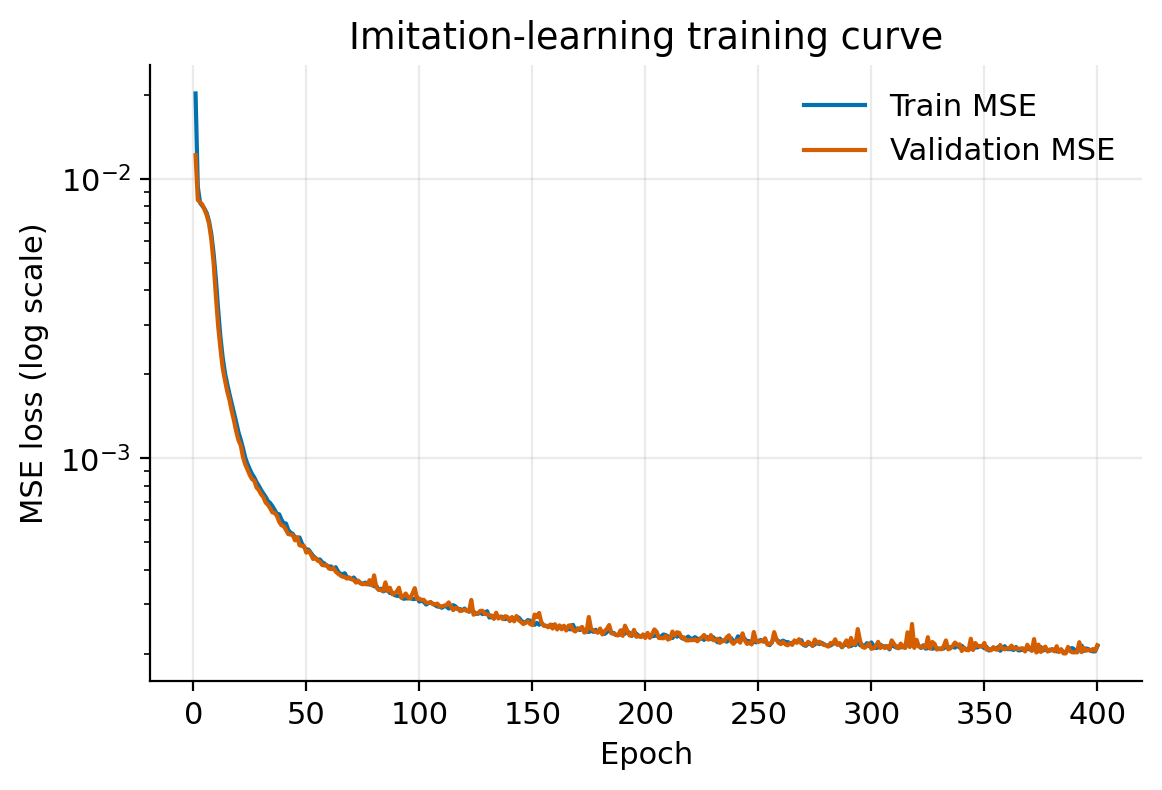
\includegraphics[width=0.68\textwidth]{fig5_training_history.png}
\caption{Imitation-learning training curve (log scale). Train and validation
MSE descend together to $\approx2.1\times10^{-4}$ with no divergence: the
network fits the optimal policy well in action space. Its economic failure
(Section~\ref{sec:results}) is therefore structural, not a training
pathology.}
\label{fig:training}
\end{figure}

% ================================================================ Results
\section{Experimental Results}
\label{sec:results}

\subsection{No-trade regions}
Figure~\ref{fig:notrade} shows the optimal no-trade region across the horizon.
For most of the horizon it is a narrow, nearly constant band around
$w^{*}=0.30$; at $t=0$ it is $[\,0.235,\ 0.365\,]$ (width $0.130$). Near the
terminal date the band flares open --- the \emph{horizon effect} --- because
with little time remaining there is too little expected benefit from
re-optimizing the allocation to justify paying the cost. Figure~\ref{fig:policy}
displays the policy slices $y^{*}(x)$, exhibiting the bang-bang-to-boundary
structure of \eqref{eq:bangbang}: flat at the lower edge, the identity $y=x$
inside the band, flat at the upper edge.

\begin{figure}[t]
\centering
\begin{subfigure}{0.49\textwidth}
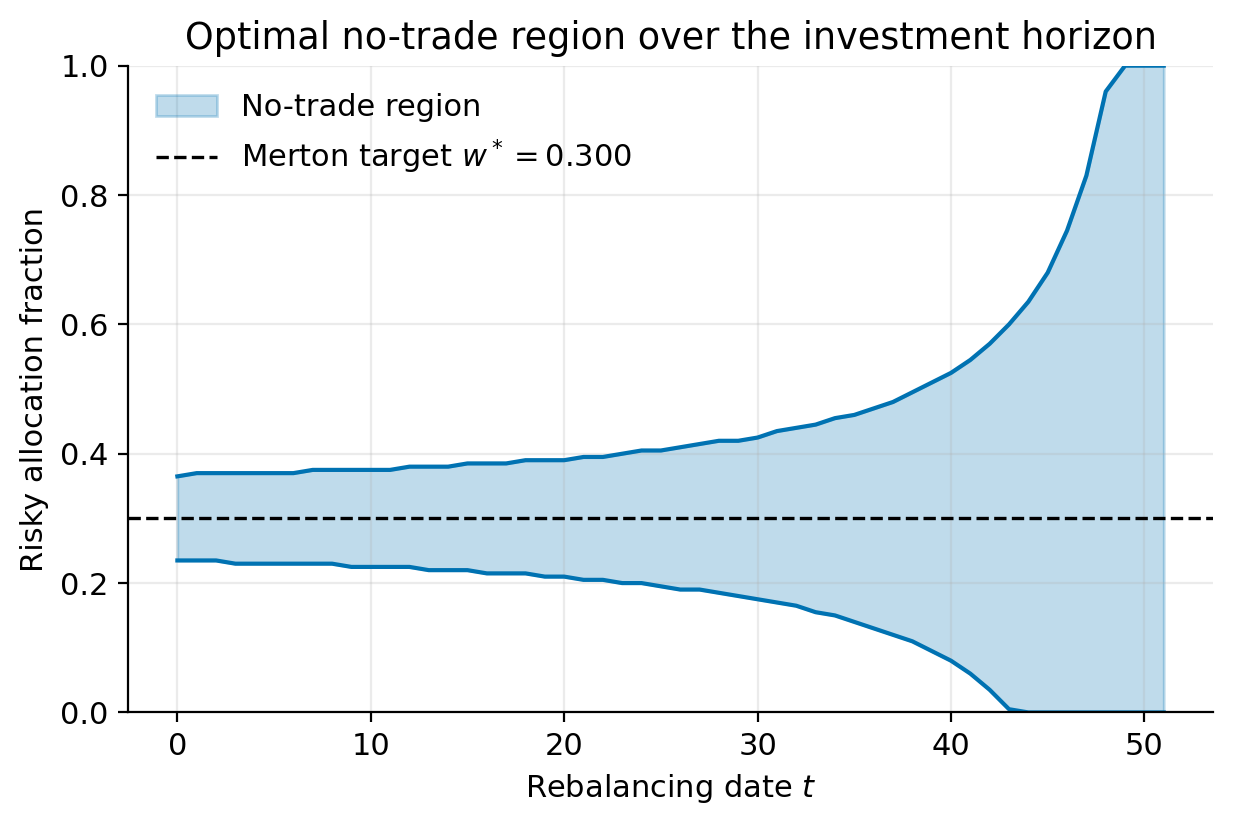
\includegraphics[width=\linewidth]{fig1_no_trade_region.png}
\caption{No-trade region over time.}
\label{fig:notrade}
\end{subfigure}\hfill
\begin{subfigure}{0.49\textwidth}
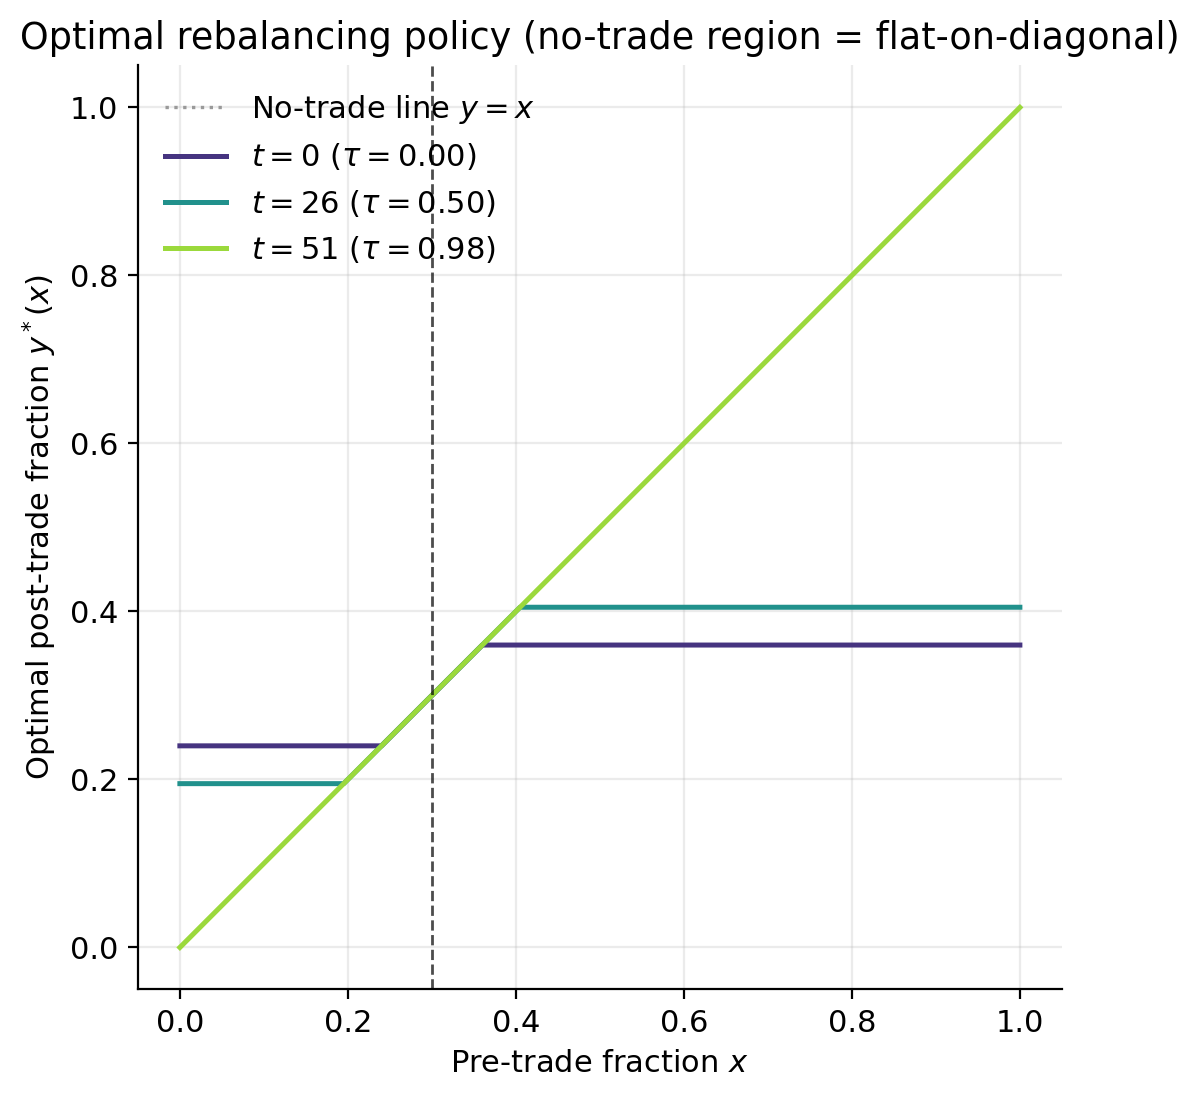
\includegraphics[width=\linewidth]{fig2_policy_slices.png}
\caption{Optimal policy $y^{*}(x)$ at three dates.}
\label{fig:policy}
\end{subfigure}
\caption{The optimal control. The band (left) is centered on the Merton target
and widens toward the horizon; the policy (right) holds inside the band and
trades to its nearest edge outside.}
\label{fig:dp}
\end{figure}

\paragraph{Comparative statics.}
Tables~\ref{tab:band-cost} and~\ref{tab:band-gamma} (and
Figure~\ref{fig:bandcost}) report how the $t=0$ band responds to the cost rate
and to risk aversion. The band widens monotonically with $tc$ --- from width
$0.040$ at $tc=0.05\%$ to $0.330$ at $tc=3\%$. For small costs the half-width
roughly triples when $tc$ increases sixteen-fold ($0.0005\!\to\!0.002$ gives
$0.020\!\to\!0.030$, ratio $1.5\approx 4^{1/3}$), consistent with the classical
$tc^{1/3}$ small-cost asymptotics \citep{shrevesoner1994}. Raising $\gamma$
lowers the target $w^{*}$ and tightens the band (width $0.270$ at $\gamma=2$ down
to $0.070$ at $\gamma=12$): more risk-averse investors hold less of the risky
asset and tolerate smaller deviations.

\begin{table}[t]
\centering
\begin{minipage}{0.52\textwidth}
\centering
\caption{No-trade band at $t{=}0$ vs cost.}
\label{tab:band-cost}
\small
\begin{tabular}{rccc}
\toprule
$tc$ & lower & upper & width\\
\midrule
$0.0005$ & $0.280$ & $0.320$ & $0.040$\\
$0.001$  & $0.275$ & $0.325$ & $0.050$\\
$0.002$  & $0.270$ & $0.330$ & $0.060$\\
$0.005$  & $0.255$ & $0.345$ & $0.090$\\
$0.01$   & $0.235$ & $0.365$ & $0.130$\\
$0.02$   & $0.190$ & $0.415$ & $0.225$\\
$0.03$   & $0.140$ & $0.470$ & $0.330$\\
\bottomrule
\end{tabular}
\end{minipage}\hfill
\begin{minipage}{0.45\textwidth}
\centering
\caption{Band at $t{=}0$ vs risk aversion.}
\label{tab:band-gamma}
\small
\begin{tabular}{rcccc}
\toprule
$\gamma$ & $w^{*}$ & lower & upper & width\\
\midrule
$2$  & $0.750$ & $0.615$ & $0.885$ & $0.270$\\
$3$  & $0.500$ & $0.400$ & $0.600$ & $0.200$\\
$5$  & $0.300$ & $0.235$ & $0.365$ & $0.130$\\
$8$  & $0.188$ & $0.140$ & $0.235$ & $0.095$\\
$12$ & $0.125$ & $0.090$ & $0.160$ & $0.070$\\
\bottomrule
\end{tabular}
\end{minipage}
\end{table}

\begin{figure}[t]
\centering
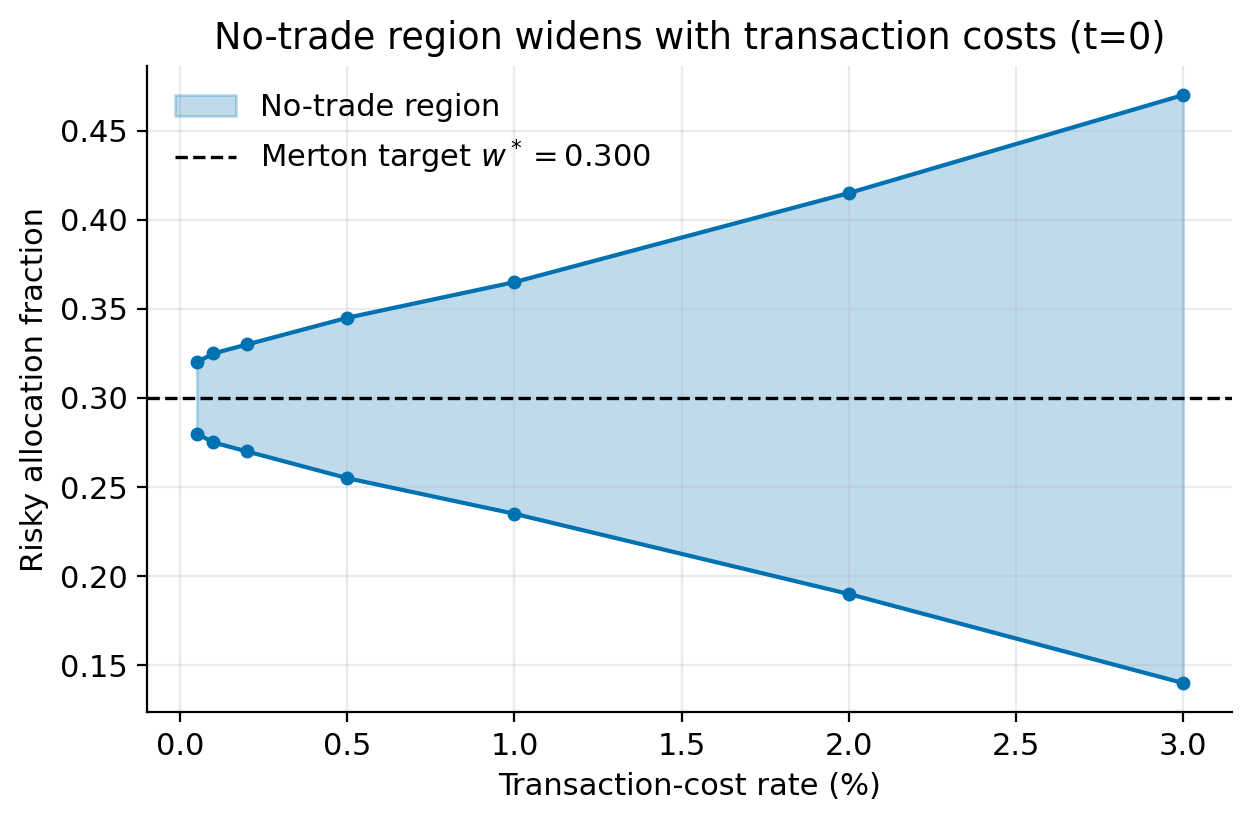
\includegraphics[width=0.62\textwidth]{fig4_band_vs_cost.png}
\caption{The no-trade region widens with the transaction-cost rate, centered on
the Merton target.}
\label{fig:bandcost}
\end{figure}

\subsection{Policy comparisons: learned vs optimal}
Figure~\ref{fig:dpml} overlays the learned policy on the optimal one. The
network captures the global shape --- low ($0.235$-like) lower plateau, diagonal
no-trade segment, upper plateau --- but \emph{smooths the kinks}. Crucially,
inside the no-trade band where the optimum is exactly $y=x$, the smooth
approximation lies slightly off the diagonal. Measured inside the $t=0$ band,
the mean residual $|y_{\mathrm{ML}}-x|$ is small but strictly positive
everywhere. Each such residual is a trade the optimal policy would not make.

\begin{figure}[t]
\centering
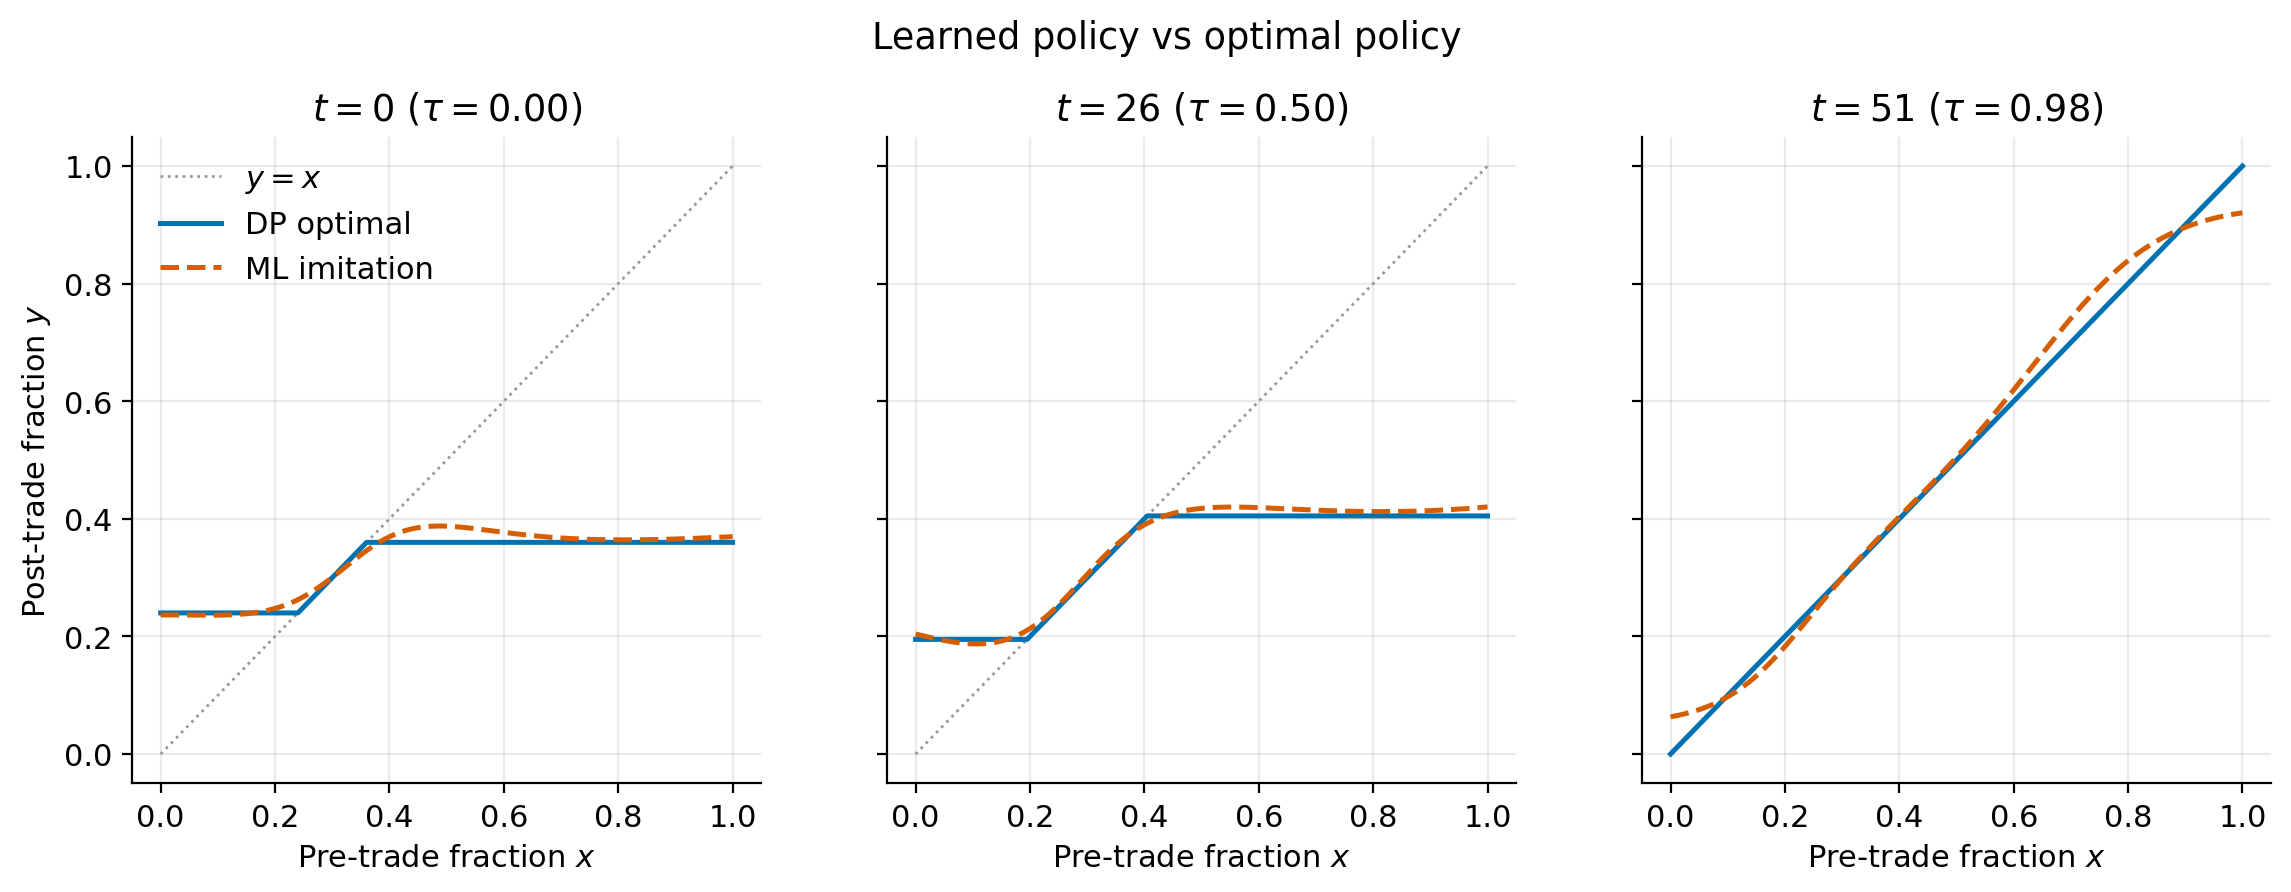
\includegraphics[width=0.95\textwidth]{fig6_dp_vs_ml_policy.png}
\caption{Learned (ML) vs optimal (DP) policy at three dates. The network smooths
the no-trade kinks; the residual off-diagonal inside the band drives spurious
trading.}
\label{fig:dpml}
\end{figure}

\subsection{Performance metrics}
We simulate all four strategies --- DP optimal, ML imitation, periodic
rebalancing (to $w^{*}$ every $4$ steps), and buy-and-hold --- on a common set of
$20{,}000$ return paths (common random numbers). Performance is summarized by the
certainty equivalent $\mathrm{CE}=\big((1-\gamma)\,\E[U(W_T)]\big)^{1/(1-\gamma)}$,
mean turnover, mean cost, and the root-mean-square action gap to the optimal
policy (tracking error). Because all strategies see identical returns, we also
report a \emph{paired} test of the per-path utility advantage of the optimal
policy, whose variance is far smaller than that of the individual estimates.

\begin{table}[t]
\centering
\caption{Performance starting \emph{at} the target ($x_0=w^{*}=0.30$),
$20{,}000$ paths. CE shown with $95\%$ confidence interval.}
\label{tab:perf-on}
\small
\begin{tabular}{lcccccc}
\toprule
Strategy & CE & $95\%$ CI & $\E[W_T]$ & Turnover & Cost & Track.\ err.\\
\midrule
DP optimal   & $1.02927$ & $[1.02842,1.03013]$ & $1.0390$ & $0.00003$ & $4\!\times\!10^{-7}$ & ---\\
Buy \& hold  & $1.02927$ & $[1.02842,1.03013]$ & $1.0390$ & $0.00000$ & $0$ & $0.0002$\\
Periodic     & $1.02821$ & $[1.02735,1.02908]$ & $1.0375$ & $0.1119$  & $0.00114$ & $0.0056$\\
ML imitation & $1.02606$ & $[1.02500,1.02713]$ & $1.0402$ & $0.2141$  & $0.00217$ & $0.0052$\\
\bottomrule
\end{tabular}
\end{table}

\begin{table}[t]
\centering
\caption{Performance starting \emph{off} the target ($x_0=0.80$),
$20{,}000$ paths.}
\label{tab:perf-off}
\small
\begin{tabular}{lcccccc}
\toprule
Strategy & CE & $95\%$ CI & $\E[W_T]$ & Turnover & Cost & Track.\ err.\\
\midrule
DP optimal   & $1.02393$ & $[1.02293,1.02494]$ & $1.0372$ & $0.4526$ & $0.00453$ & ---\\
Buy \& hold  & $1.02378$ & $[1.02292,1.02464]$ & $1.0337$ & $0.5000$ & $0.00500$ & $0.0083$\\
Periodic     & $1.02269$ & $[1.02183,1.02356]$ & $1.0320$ & $0.6120$ & $0.00614$ & $0.0100$\\
ML imitation & $1.02063$ & $[1.01956,1.02171]$ & $1.0351$ & $0.7065$ & $0.00709$ & $0.0065$\\
\bottomrule
\end{tabular}
\end{table}

\begin{table}[t]
\centering
\caption{Paired utility advantage of the DP-optimal policy (common random
numbers). Positive means DP is better; $t$-statistics in the final column.}
\label{tab:paired}
\small
\begin{tabular}{llccc}
\toprule
Start & DP vs & Mean adv.\ ($\times10^{3}$) & $t$-stat & DP better @ $95\%$\\
\midrule
on-target  & ML imitation & $+2.799$ & $20.1$  & yes\\
on-target  & Periodic     & $+0.918$ & $24.1$  & yes\\
on-target  & Buy \& hold  & $-0.0001$& $-0.4$  & no (tie)\\
\midrule
off-target & ML imitation & $+2.959$ & $28.8$  & yes\\
off-target & Periodic     & $+1.108$ & $17.0$  & yes\\
off-target & Buy \& hold  & $+0.140$ & $2.0$   & yes\\
\bottomrule
\end{tabular}
\end{table}

\begin{figure}[t]
\centering
\begin{subfigure}{0.46\textwidth}
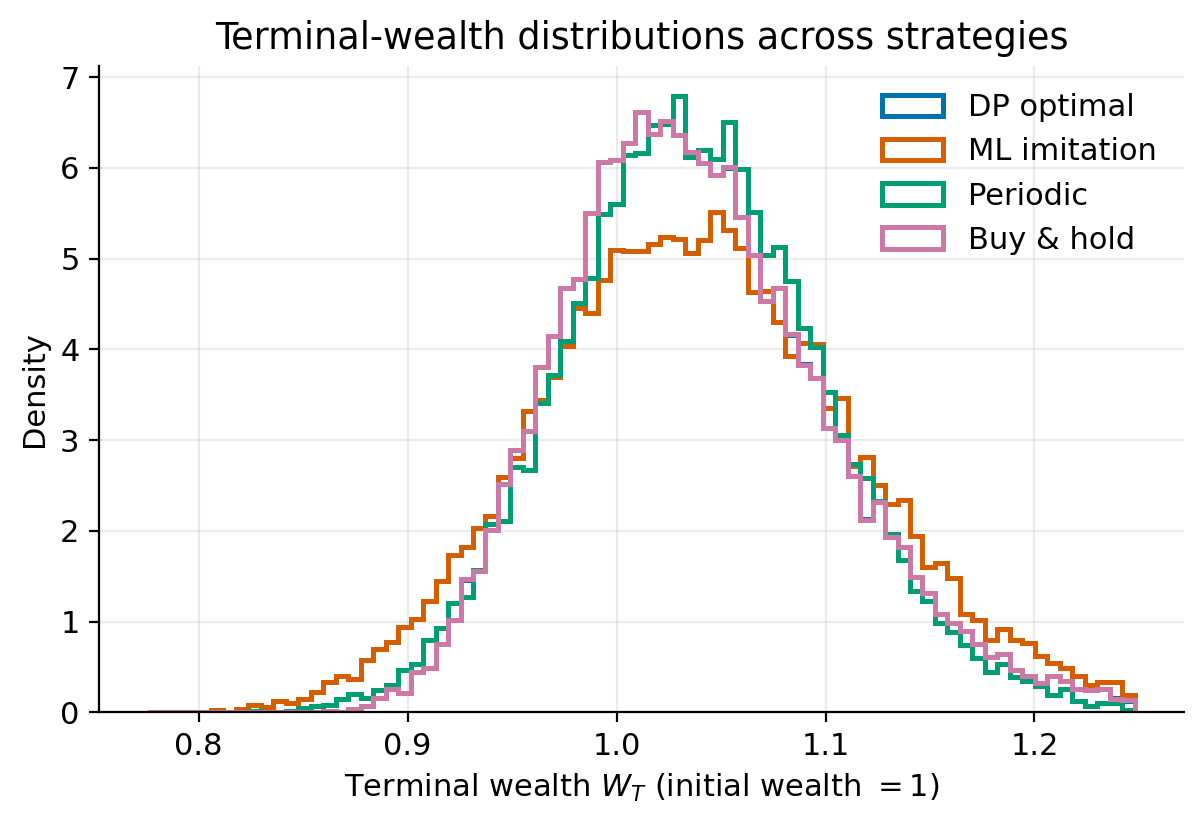
\includegraphics[width=\linewidth]{fig7_wealth_distributions.png}
\caption{Terminal-wealth distributions.}
\end{subfigure}\hfill
\begin{subfigure}{0.53\textwidth}
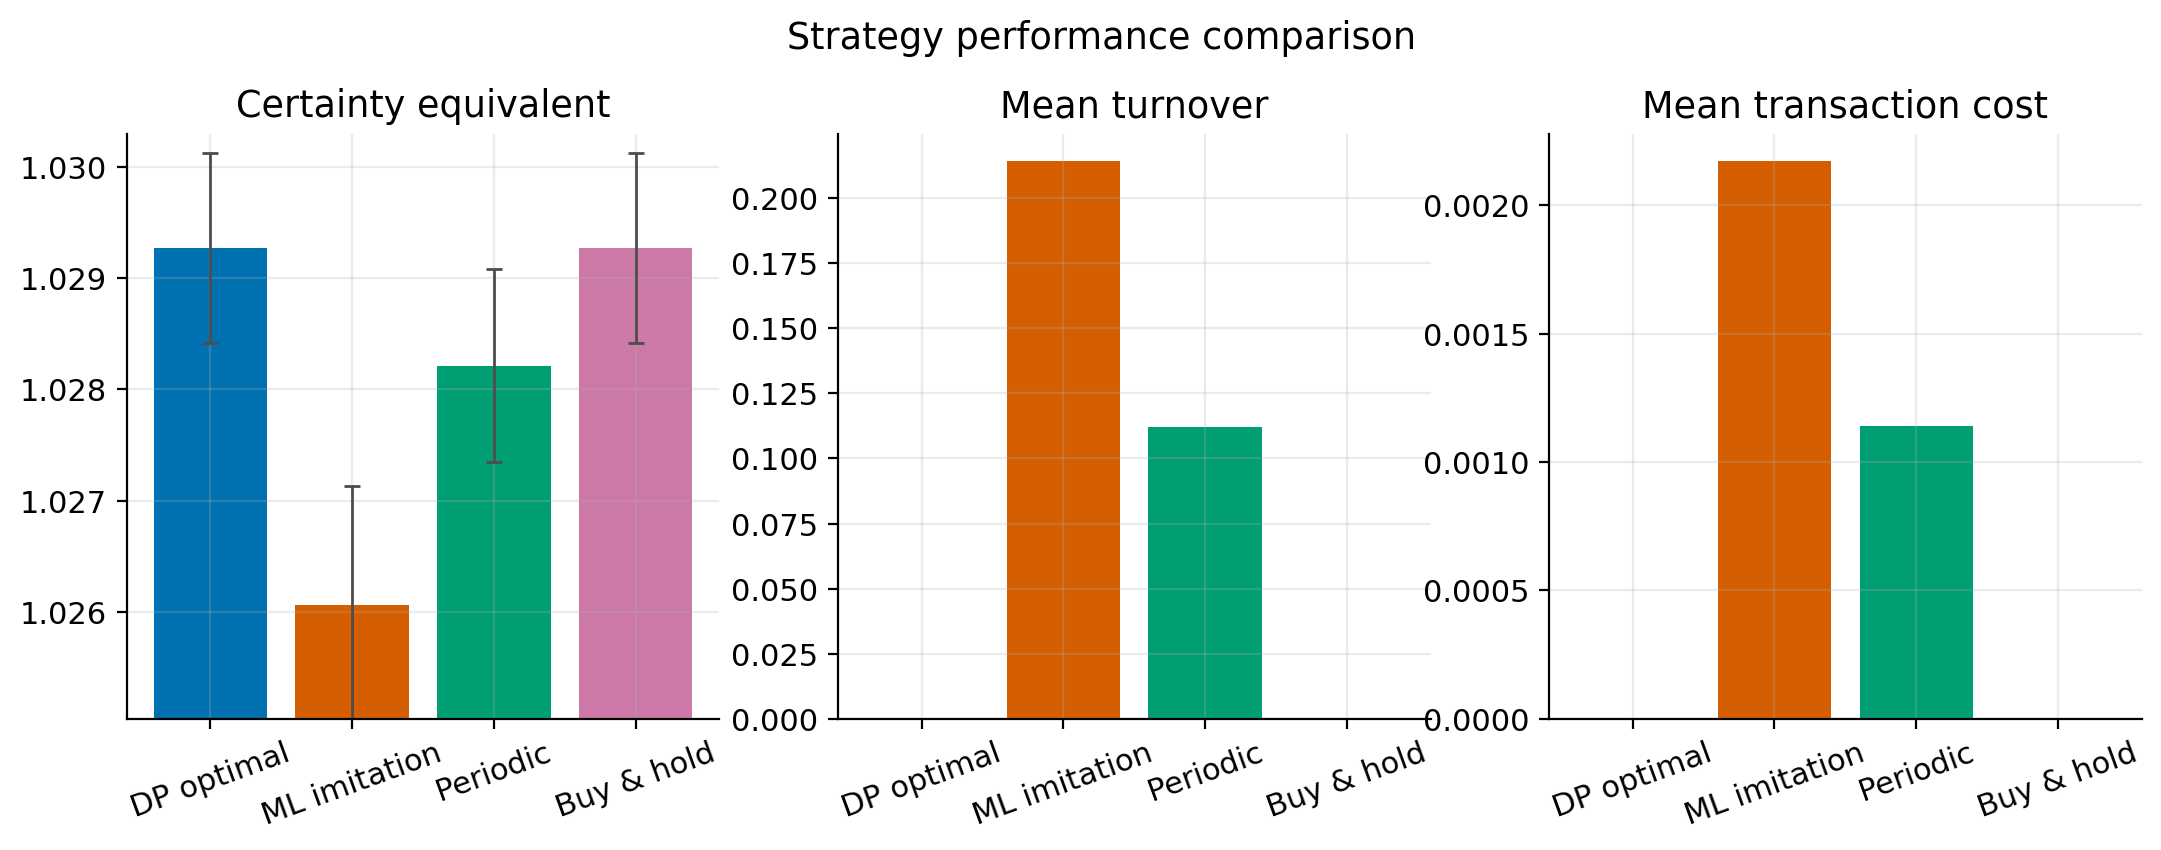
\includegraphics[width=\linewidth]{fig8_performance_bars.png}
\caption{CE (with $95\%$ CI), turnover, cost.}
\end{subfigure}
\caption{Strategy comparison on a common set of paths (on-target start).}
\label{fig:perf}
\end{figure}

Three findings emerge (Tables~\ref{tab:perf-on}--\ref{tab:paired},
Figure~\ref{fig:perf}).
\begin{enumerate}
\item \textbf{The DP policy is optimal, as it must be.} It attains the highest
certainty equivalent and dominates ML and periodic rebalancing with large
$t$-statistics ($20$--$29$). When the portfolio starts \emph{on} target it ties
buy-and-hold ($t=-0.4$, not significant): a wide no-trade band makes optimal
behavior essentially ``do nothing,'' so the do-nothing heuristic is optimal
here. Starting \emph{off} target, the optimal policy beats every baseline
including buy-and-hold, trading in most cost-efficiently (turnover $0.45$ vs
$0.50$ for buy-and-hold and $0.61$ for periodic).
\item \textbf{Naive imitation is the worst strategy.} Despite a tiny validation
MSE and a small tracking error ($0.005$), the ML policy has by far the highest
turnover ($0.21$ vs $3\times10^{-5}$ for DP) and cost, and the lowest certainty
equivalent. The smooth network cannot reproduce the exact $y=x$ identity on the
positive-measure no-trade region, so it trades \emph{continuously} where the
optimum holds.
\item \textbf{Low action error $\ne$ good control.} The disconnect between ML's
low tracking error and poor economic performance is the paper's central lesson:
errors inside the inaction region are economically amplified into turnover and
cost, a structure invisible to an action-space MSE objective.
\end{enumerate}

\subsection{Repairing the imitation}
\label{sec:remedies}
A diagnosis is worth little unless it predicts a fix. If the failure really is
the missing inaction region --- and not capacity, optimization, or
generalization --- then restoring that region should recover the lost
performance, and nothing else should be required. We test two ways of doing so.

\paragraph{A dead-zone wrapper (inference time).}
Leave the trained network untouched and snap small predicted trades to exact
inaction:
\begin{equation}
y=\begin{cases}
x, & |\hat y(t,x)-x|\le\delta,\\[2pt]
\hat y(t,x), & \text{otherwise.}
\end{cases}
\label{eq:deadzone}
\end{equation}
Returning $x$ \emph{exactly} is what matters: cost is charged on any deviation,
so only an exact match is genuinely free. This restores an inaction region of
half-width $\delta$ by construction, costs nothing to train, and adds one
comparison per step.

\paragraph{A cost-aware objective (training time).}
Alternatively, charge the student during training for trading more than its
teacher does:
\begin{equation}
\mathcal{L}=\mathrm{MSE}(\hat y,y^{*})
+\lambda\,\E\big[(\,|\hat y-x|-|y^{*}-x|\,)^{+}\big].
\label{eq:costaware}
\end{equation}
The asymmetry is deliberate. Penalizing $|\hat y-x|$ outright would also
discourage the large, correct trades made from outside the band, biasing the
student toward inaction everywhere. Penalizing only the \emph{excess} over the
teacher's own trade size leaves correct trading unpunished and bills the student
exactly for the spurious turnover it invents inside the band. We use
$\lambda=1$.

\begin{table}[t]
\centering
\caption{Repairing the learned policy, on-target start, $20{,}000$ paths and the
same return paths as Table~\ref{tab:perf-on}. ``Gap closed'' is the fraction of
the DP--ML certainty-equivalent gap ($3.208\times10^{-3}$) recovered. The final
column is the paired $t$-statistic against the DP optimum; small values mean the
policy is no longer statistically distinguishable from optimal.}
\label{tab:remedies}
\small
\begin{tabular}{lcccc}
\toprule
Policy & CE & Turnover & Gap closed & $t$ vs DP\\
\midrule
DP optimal                     & $1.029272$ & $3.4\!\times\!10^{-5}$ & ---      & ---\\
ML imitation                   & $1.026064$ & $0.2141$               & $0\%$    & $20.1$\\
\midrule
\ \ $+$ dead-zone $\delta=0.002$ & $1.026175$ & $0.2032$             & $3.5\%$  & $19.4$\\
\ \ $+$ dead-zone $\delta=0.005$ & $1.026602$ & $0.1714$             & $16.8\%$ & $18.4$\\
\ \ $+$ dead-zone $\delta=0.01$  & $1.027331$ & $0.1277$             & $39.5\%$ & $18.4$\\
\ \ $+$ dead-zone $\delta=0.02$  & $1.029146$ & $0.0083$             & $96.1\%$ & $7.7$\\
\ \ $+$ dead-zone $\delta=0.05$  & $\mathbf{1.029272}$ & $9\!\times\!10^{-17}$ & $\mathbf{100\%}$ & $\mathbf{-0.4}$\\
\midrule
ML cost-aware                  & $1.027807$ & $0.1065$               & $54.3\%$ & $17.4$\\
\ \ $+$ dead-zone $\delta=0.01$  & $\mathbf{1.029272}$ & $4.8\!\times\!10^{-5}$ & $\mathbf{100\%}$ & $2.1$\\
\bottomrule
\end{tabular}
\end{table}

\begin{figure}[t]
\centering
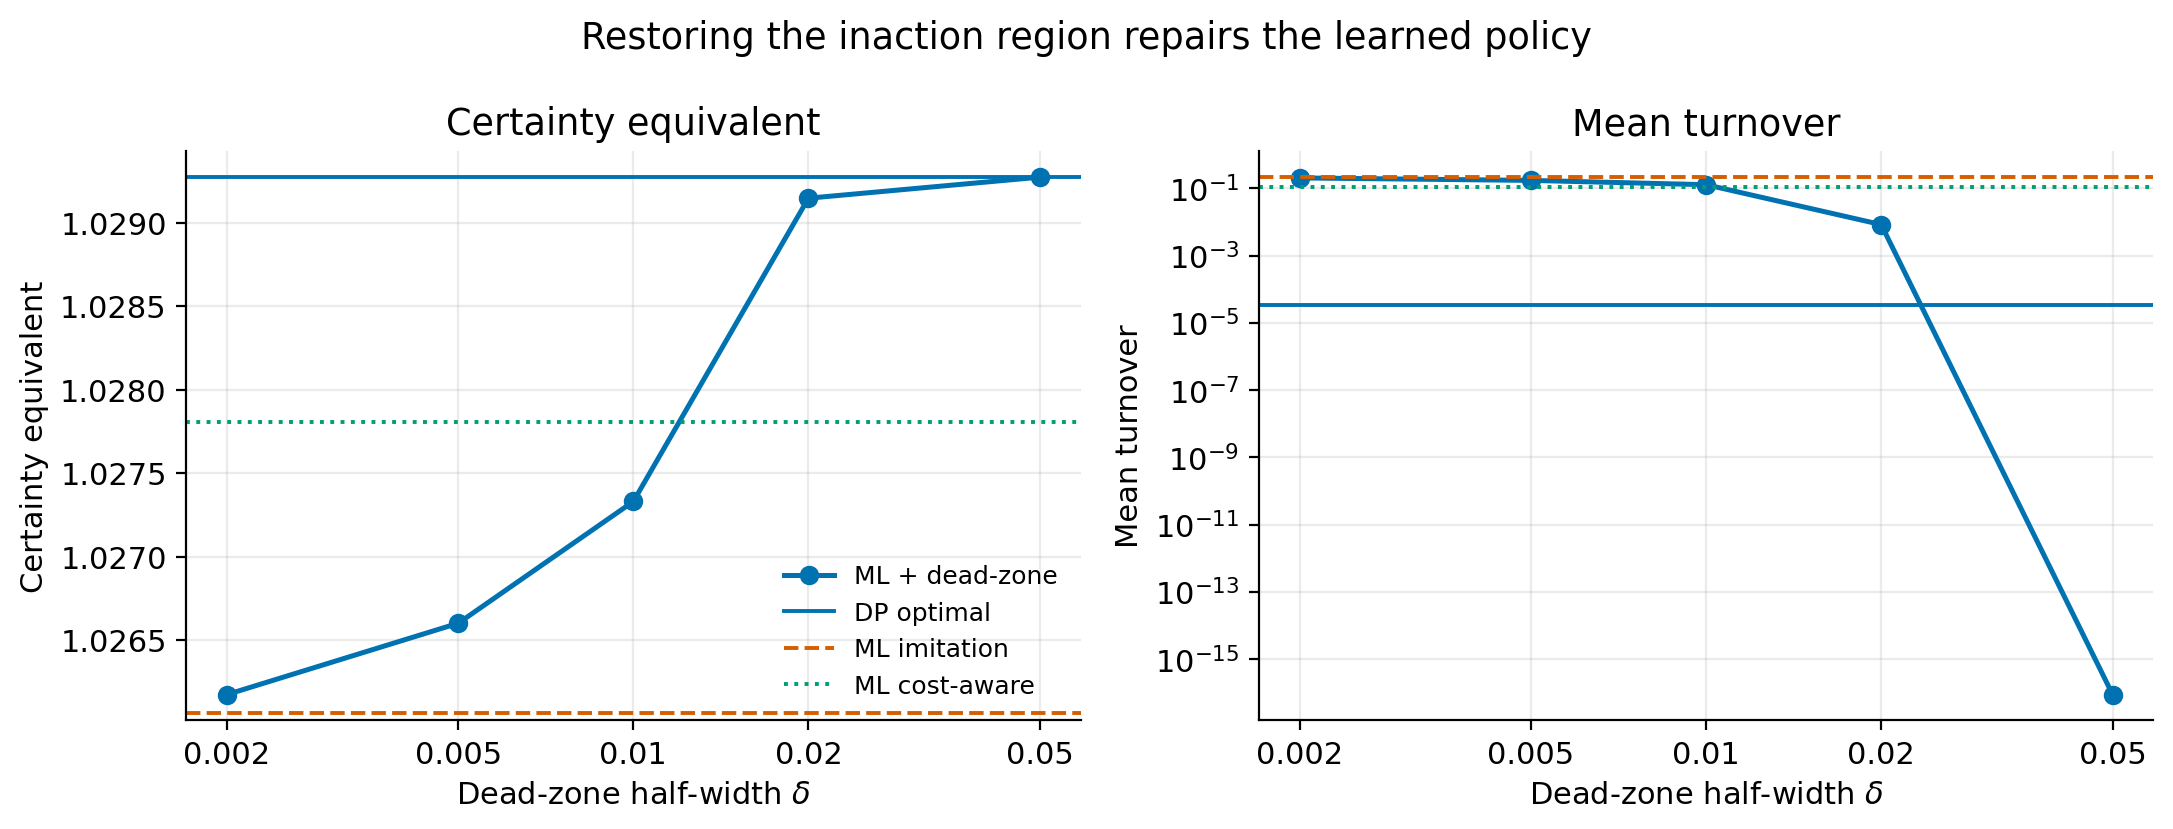
\includegraphics[width=0.95\textwidth]{fig9_remedies.png}
\caption{Certainty equivalent and turnover of the dead-zone-wrapped policy as
$\delta$ varies, against the DP optimum and the two ML endpoints. The transition
occurs where $\delta$ crosses the network's in-band residual.}
\label{fig:remedies}
\end{figure}

Table~\ref{tab:remedies} and Figure~\ref{fig:remedies} report the outcome, and
it is unambiguous.

\begin{enumerate}
\item \textbf{The dead-zone recovers the optimum exactly.} At $\delta=0.05$ the
learned policy attains a certainty equivalent of $1.029272$ --- the DP value to
six decimals --- with turnover of $9\times10^{-17}$, i.e.\ it stops trading
altogether when it should. The paired test against the optimum gives
$t=-0.4$: after the repair, the network is \emph{no longer statistically
distinguishable from the optimal control}, having been beaten at $t=20.1$
before it.
\item \textbf{The transition is where the mechanism says it should be.} The
network's mean in-band residual is $9.6\times10^{-3}$. Dead-zones below that
value do essentially nothing ($3.5\%$ of the gap at $\delta=0.002$); the
recovery happens as $\delta$ crosses it ($39.5\%$ at $\delta=0.01$, $96.1\%$ at
$\delta=0.02$, $100\%$ at $\delta=0.05$). The fix works exactly when it covers
the defect it was designed for, which is the strongest evidence we can offer
that the diagnosis is the right one.
\item \textbf{The cost-aware loss attacks the same quantity, from the other
side.} It shrinks the in-band residual from $9.6\times10^{-3}$ to
$2.6\times10^{-3}$, a factor of $3.8$, and closes $54.3\%$ of the gap on its own
with no wrapper at all. Combined, the two are complementary: because the
residual is smaller, a dead-zone \emph{five times tighter} ($\delta=0.01$)
suffices to reach the optimum.
\item \textbf{$\delta$ is a real trade-off, not a free parameter.} A dead-zone
wide enough to cover the residual also suppresses genuine rebalancing. Starting
off-target the same $\delta=0.05$ closes $99.2\%$ rather than $100\%$ of the
gap, and under-trades relative to the optimum (turnover $0.438$ versus $0.453$);
pushed far enough, a dead-zone simply refuses to correct a bad allocation. This
is why the cost-aware loss matters: it buys the same repair at a tighter, safer
$\delta$.
\end{enumerate}

\noindent
The practical reading is that neither remedy is exotic --- one is three lines at
inference, the other one term in the loss --- and either is enough to turn the
worst strategy in Table~\ref{tab:perf-on} into one that ties the optimum. What
they have in common is that both encode the inaction structure rather than
hoping the regressor will discover it.

\subsection{Is the failure robust, or is it one unlucky fit?}
\label{sec:robustness}
Everything so far rests on a single trained network. That is enough to
\emph{describe} a failure but not to establish one: the obvious objection is
that we happened to train a bad student. We therefore repeat the imitation
experiment across $10$ independent training seeds at the published architecture,
and across $7$ architectures at the base seed, spanning $337$ to $66{,}817$
parameters --- a factor of $198$ in capacity. All $17$ students are evaluated on
the same $20{,}000$ paths as Table~\ref{tab:perf-on}, against the same teacher,
which is seed-independent and solved once.

\paragraph{Across seeds.}
Every one of the $10$ retrainings fits well and behaves badly. Validation MSE
stays in $[1.65,2.50]\times10^{-4}$; the in-band residual is
$1.10\times10^{-2}\pm1.4\times10^{-3}$; realized turnover is
$0.236\pm0.039$ against the optimal policy's $3.4\times10^{-5}$; and the
certainty equivalent lies in $[1.02437,1.02662]$, \emph{below the DP optimum of
$1.02927$ in $10$ cases out of $10$}. There is no seed at which naive imitation
is competitive. The mean certainty-equivalent shortfall is
$3.41\times10^{-3}$, close to the $3.21\times10^{-3}$ of the headline run, so
the paper's single-seed result is typical rather than extreme.

\begin{table}[t]
\centering
\caption{The failure across architectures (base seed, $20{,}000$ paths). Capacity
spans a factor of $198$ and depth ranges from two to four hidden layers. Every
row under-performs the DP optimum ($\mathrm{CE}=1.02927$); every row repairs to
it exactly under a $\delta=0.05$ dead-zone.}
\label{tab:robustness}
\small
\begin{tabular}{lrcccc}
\toprule
Architecture & Params & Val.\ MSE & In-band $|\hat y-x|$ & Turnover & CE\\
\midrule
$16\times16$    & $337$    & $2.18\!\times\!10^{-4}$ & $0.01043$ & $0.2596$ & $1.02532$\\
$32\times32$    & $1{,}185$ & $2.34\!\times\!10^{-4}$ & $0.00903$ & $0.2750$ & $1.02478$\\
$64\times64$    & $4{,}417$ & $2.14\!\times\!10^{-4}$ & $0.00961$ & $0.2141$ & $1.02606$\\
$128\times128$  & $17{,}025$ & $2.01\!\times\!10^{-4}$ & $0.01251$ & $0.2019$ & $1.02632$\\
$256\times256$  & $66{,}817$ & $2.08\!\times\!10^{-4}$ & $\mathbf{0.01662}$ & $0.2668$ & $1.02544$\\
$64\times64\times64$ & $8{,}577$ & $9.83\!\times\!10^{-5}$ & $0.00751$ & $0.1806$ & $1.02672$\\
$64\times64\times64\times64$ & $12{,}737$ & $\mathbf{8.92\!\times\!10^{-5}}$ & $0.00799$ & $0.2147$ & $1.02649$\\
\midrule
DP optimal & --- & --- & $0$ (exactly) & $0.00003$ & $\mathbf{1.02927}$\\
\bottomrule
\end{tabular}
\end{table}

\paragraph{Across architectures.}
Table~\ref{tab:robustness} makes the sharper point. Capacity does not help, and
the two natural ``just train a better network'' responses both fail.
\begin{enumerate}
\item \textbf{More parameters do not restore inaction.} The $256\times256$
network has $198$ times the parameters of the $16\times16$ network and a
\emph{larger} in-band residual ($0.01662$ versus $0.01043$, a factor of $1.59$
in the wrong direction). Across the whole sweep the residual never falls below
$7.5\times10^{-3}$ and shows no downward trend in capacity. This is what the
representational argument predicts: the obstruction is that a smooth function
cannot equal the identity on a positive-measure set, and no amount of width
changes that.
\item \textbf{Fitting better does not control better.} The best fit in the
entire study is the four-layer network, whose validation MSE of
$8.92\times10^{-5}$ is $2.4$ times smaller than the published run's. It still
turns over $0.215$ and still loses to the optimum. Ranking the seventeen
students by validation error tells you essentially nothing about their
economics --- which is the paper's central lesson, now stated over a population
of fits rather than a single one.
\end{enumerate}

\paragraph{The repair is equally universal.}
Applying the $\delta=0.05$ dead-zone of Equation~\eqref{eq:deadzone} to each of
the $17$ students, every one attains a certainty equivalent of $1.02927$ --- the
DP value, to five decimals, in all seventeen cases --- with residual turnover of
at most $2.6\times10^{-6}$. The repair is not tuned per fit and does not depend
on the architecture or the seed. Both the disease and the cure are properties of
the control problem, not of any particular network.

\begin{figure}[t]
\centering
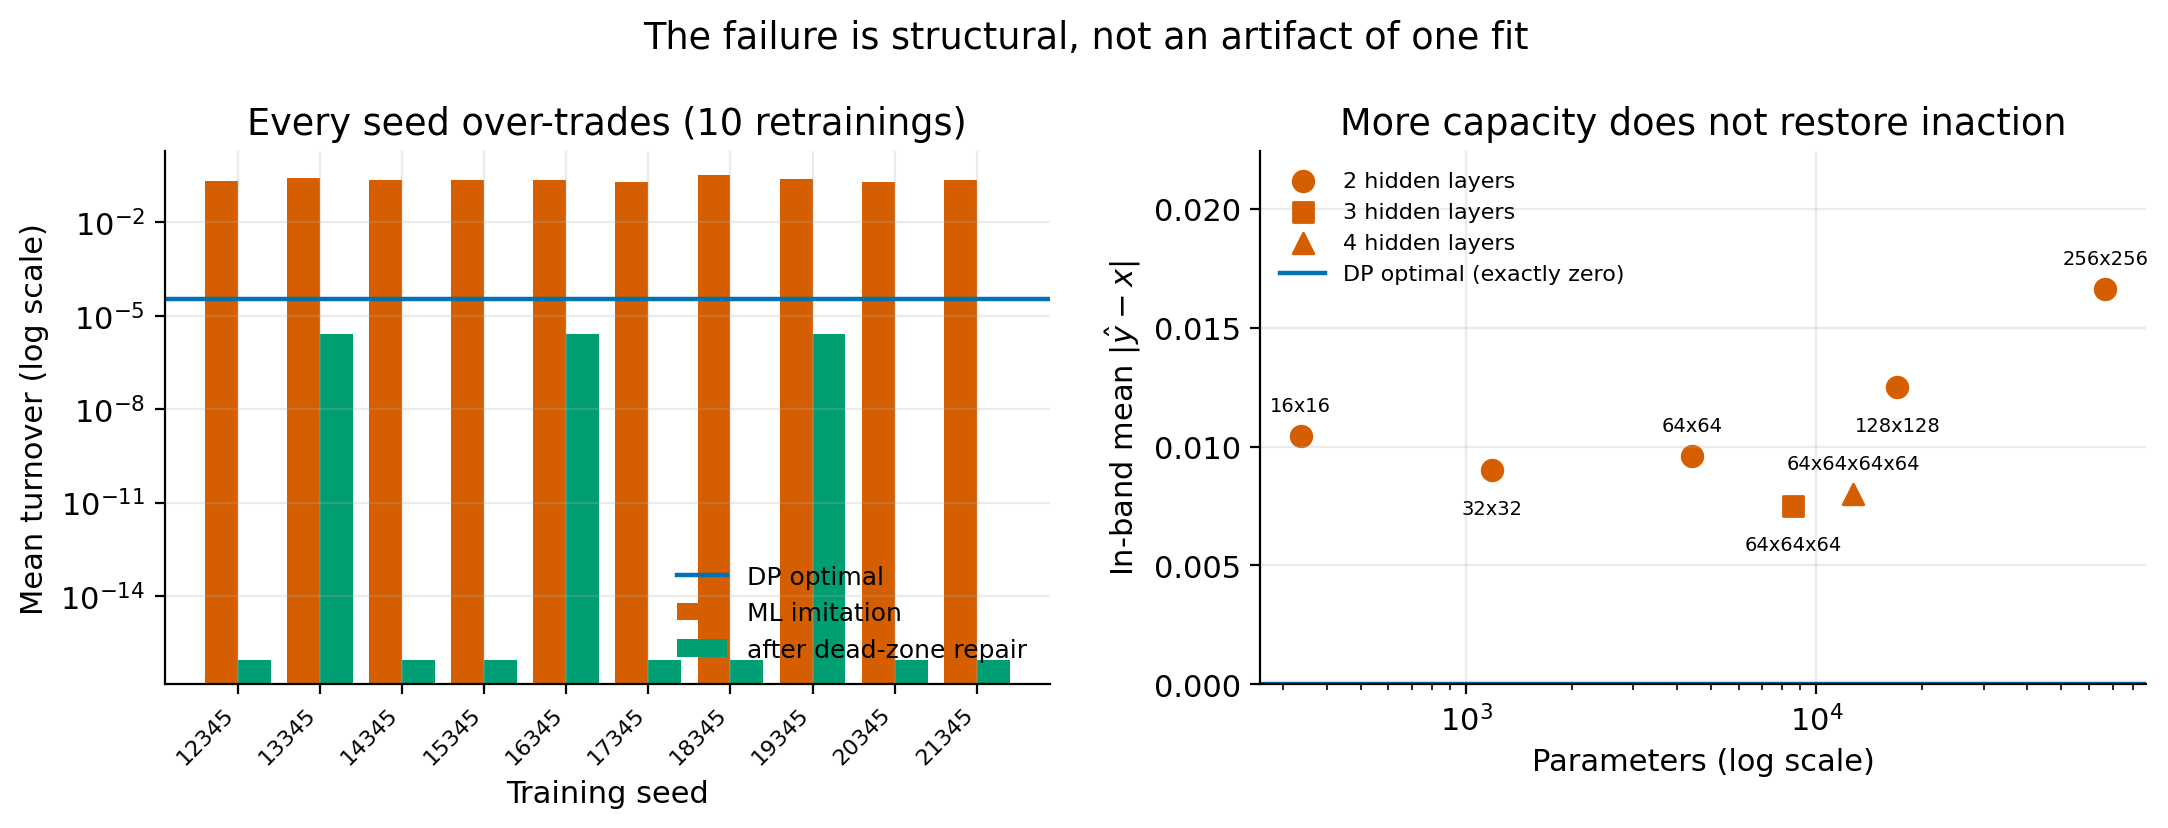
\includegraphics[width=0.95\textwidth]{fig10_robustness.png}
\caption{Left: realized turnover for each of the $10$ retraining seeds, before
and after the dead-zone repair, against the optimal policy. Right: in-band
residual against parameter count; the horizontal line at zero is the optimal
policy, which the students never approach at any capacity.}
\label{fig:robustness}
\end{figure}

% ================================================================ Discussion
\section{Discussion}

\paragraph{Interpretation of the learned policy.}
The failure mode is not a capacity or optimization problem --- the network fits
the policy well in MSE, and Section~\ref{sec:robustness} shows that neither more
parameters nor a better fit rescues it --- but a \emph{representational mismatch} with the
geometry of optimal control. Optimal rebalancing is governed by a free boundary
(the band edges) and an identity map in between. A smooth regressor approximates
the identity map with a wiggle, and because the wealth dynamics charge cost on
\emph{any} deviation, a wiggle of size $\varepsilon$ produces turnover of order
$\varepsilon$ per step, accumulating to first order in $N$ while the utility
benefit of being marginally better allocated is only second order. Hence small
$\varepsilon$ still hurts.

\paragraph{Remedies.}
Two cheap fixes follow directly from this diagnosis, and
Section~\ref{sec:remedies} shows both work: a \emph{dead-zone} wrapper that
snaps small predicted trades to exact inaction, and a \emph{cost-aware loss}
that charges the student for trading beyond its teacher. Either closes the
entire certainty-equivalent gap, and the dead-zone begins to work exactly where
$\delta$ crosses the network's in-band residual --- the fix engages precisely
when it covers the defect, which is the sharpest confirmation of the mechanism
we can give. A third route we have not tested is imitation in \emph{value}
rather than action space (regress $g_t$ and act greedily), which would sidestep
the representational problem entirely by never asking a smooth function to
reproduce a kink.

\paragraph{Computational trade-offs.}
For this one-dimensional problem the DP solve is already trivial
($\approx 0.02$\,s), so ML offers no speed advantage here; its appeal is
asymptotic, in higher-dimensional settings where the DP grid is infeasible. Our
result is a cautionary calibration: before scaling imitation to many assets, the
inaction structure must be built into the hypothesis class or the loss.

\paragraph{Practical implications.}
The strong showing of buy-and-hold on a one-year horizon, and of the optimal
policy's near-inaction when started on target, both underline that \emph{the
cheapest correct action is usually to do nothing}. Turnover is a cost, not a
virtue; periodic rebalancing pays for trades the optimal policy would skip.

% ================================================================ Limitations
\section{Limitations and Future Work}

Our model is deliberately minimal. (i) \textbf{Multi-asset extension}: the
homogeneity reduction survives with multiple risky assets, but the no-trade
region becomes a multi-dimensional polytope and the grid grows exponentially ---
precisely where learned controllers should help \citep{liu2004}. (ii)
\textbf{Stochastic volatility} and predictable returns
\citep{garleanupedersen2013} would make the band time- and state-dependent in
richer ways. (iii) \textbf{Deep variational solvers}: rather than imitating a
precomputed policy, one can solve the Hamilton--Jacobi--Bellman equation directly
with neural networks \citep{hanjentzene2018} or train under a frictional P\&L
objective as in deep hedging \citep{buehler2019deephedging}, sidestepping the
teacher entirely. (iv) We use proportional costs only; fixed or quadratic costs
change the geometry (e.g.\ fixed costs induce discrete jumps to an interior
target). (v) Intermediate consumption and an infinite horizon are natural
extensions of the present terminal-wealth formulation.

(vi) The robustness study of Section~\ref{sec:robustness} varies the seed and
the architecture but not the \emph{model class}: every student is a feedforward
MLP trained by regression on the policy. Architectures with built-in
discontinuities (ReLU networks with learned thresholds, mixture-of-experts
gating, or an explicit hold/trade classification head) might represent the
inaction region natively, and our result should not be read as a claim about all
learned controllers --- only about smooth action-space regression, which is the
default choice.

Above all, (vii) \textbf{there is no empirical component}. Returns are simulated
from the assumed geometric Brownian motion and the parameters are stylized
rather than estimated, so the paper offers no evidence that the bands reported
here are the right bands for any actual portfolio. Real returns are not
lognormal --- they are fat-tailed, volatility-clustered and serially dependent
--- and real execution costs are neither purely proportional nor constant across
trade sizes. Confronting the solver with historical prices, estimating $\mu$ and
$\sigma$ with their sampling error propagated into the band, and measuring
realized turnover against a live cost model are all necessary before any of the
numbers here could guide an allocation decision. We regard that as the natural
next step rather than a defect of the present exercise, whose aim is to
establish the structure of the control problem and the failure mode of naive
imitation.

% ================================================================ Conclusion
\section{Conclusion}

We formulated portfolio rebalancing under proportional transaction costs as a
finite-horizon stochastic control problem, reduced it to one dimension via CRRA
homogeneity, and solved it exactly by backward induction. The solver reproduces
the classical no-trade region and its comparative statics --- widening with cost
($\sim tc^{1/3}$), narrowing with risk aversion, and flaring near the horizon.
Testing a lightweight neural network as a fast approximate controller, we found
that naive supervised imitation, though accurate in mean-squared action error,
is the worst-performing strategy because it cannot represent the no-trade region
and therefore over-trades. Crucially, the diagnosis proved actionable: encoding
the inaction region --- either as a dead-zone wrapper at inference or as an
excess-turnover penalty in the loss --- closed the entire certainty-equivalent
gap and left the repaired policy statistically indistinguishable from the
optimal control, with the recovery setting in exactly where the dead-zone width
crosses the network's in-band residual. The lesson generalizes beyond this
model: imitating optimal control requires encoding the inaction structure, not
merely minimizing action error, and doing so is cheap once the failure is
understood. All figures, tables, and checkpoints are reproducible from the
accompanying code via a single command.

% ================================================== Reproducibility
\section*{Reproducibility and code availability}
\addcontentsline{toc}{section}{Reproducibility and code availability}

Every number, table and figure in this paper is regenerated by two commands:
\begin{itemize}
\setlength{\itemsep}{2pt}
\item \texttt{python scripts/run\_all.py} --- the solver, the imitation study
and the remedies of Section~\ref{sec:remedies}; about $40$ seconds on a laptop
CPU.
\item \texttt{python scripts/run\_robustness.py} --- the seed and architecture
sweep of Section~\ref{sec:robustness}, which retrains the network seventeen
times; about seven minutes.
\end{itemize}
\noindent
All randomness derives from one seed (\texttt{Config.seed}
$=12345$) and all economic and numerical parameters live in a single
\texttt{Config} dataclass, so the run is deterministic: repeated executions
reproduce the committed tables, checkpoints and figures \emph{byte for byte}.
The only artifacts excluded from that guarantee are wall-clock timings, which
are machine-dependent and are written to a separate file rather than mixed
into the metrics.

The repository ships an automated test suite (\texttt{pytest}) that checks the
claims made here rather than merely exercising the code. It verifies the
quadrature against the analytic lognormal moments; the proportional-cost
identity of Proposition~\ref{prop:m}, including that no-trade is exactly
costless; that the no-trade band brackets the Merton fraction, widens
monotonically with $tc$ at a fitted log--log slope consistent with the
$tc^{1/3}$ asymptotics, narrows with $\gamma$, and collapses to the Merton
point when $tc=0$; that the band is stable under grid and quadrature
refinement; that the learned policy is off the $y=x$ diagonal at
\emph{every} point inside the band, which is the mechanism of
Section~\ref{sec:results}; and that every figure, table entry and quoted
statistic in this manuscript agrees with the generated results file. The
environment the reported numbers were produced in (Python 3.10.11, NumPy
1.26.4, SciPy 1.15.3, PyTorch 2.7.1, CPU only) is pinned in
\texttt{requirements-lock.txt}.

% ================================================== Declarations
\section*{Declarations}
\addcontentsline{toc}{section}{Declarations}

\paragraph{Code availability.}
All code needed to regenerate every figure, table and number in this paper is
openly available at \coderepo, archived at \codedoi. The repository contains the
solver, the training and evaluation pipeline, the manuscript source, and an
automated test suite; \texttt{python scripts/run\_all.py} reproduces the
complete set of results, and \texttt{pytest} verifies both the numerical claims
and the agreement between this manuscript and the generated results.

\paragraph{Data availability.}
This study generated and analysed no empirical data. Every return path is
simulated from the model of Equation~\eqref{eq:gbm} under a single fixed seed,
as described in Section~\ref{sec:numerics}; the simulated data are therefore
fully specified by the parameters of Table~\ref{tab:params} and are regenerated
deterministically by the code above rather than distributed as files.

\paragraph{Funding.}
This research received no specific grant from any funding agency in the public,
commercial or not-for-profit sectors.

\paragraph{Competing interests.}
The author declares no competing interests.

\paragraph{Author contributions.}
The author is solely responsible for the conception, implementation, analysis
and writing of this work.

\paragraph{ORCID.}
Rahul Thakur: \authororcid.

% ================================================================ Refs
\bibliographystyle{plainnat}
\bibliography{refs}

\end{document}
